\documentclass[10pt, a4paper]{article}
\usepackage[utf8]{inputenc}
\usepackage[paper=a4paper, left=3.0cm, right=3.0cm, bottom=1.5cm, top=3.5cm]{geometry}
\usepackage{mathtools}
\usepackage{float}
%\usepackage{graphicx}
\usepackage[]{algorithm2e}
\usepackage{amssymb}
\usepackage{subcaption}

\usepackage[conEntregas]{caratula}

\begin{document}

\titulo{Trabajo Pr\'actico 1}

\fecha{10/04/2015}

\materia{Introducción al Procesamiento Digital de Imágenes}

\integrante{Dellanzo, Claudia Antonella}{019/13}{antodellanzo@gmail.com}
\integrante{Julián Bayardo}{850/13}{julian@bayardo.info}
% Pongan cuantos integrantes quieran

\maketitle
\tableofcontents

\newpage

\section{Introducción}

El objetivo de este trabajo prático es implementar un algoritmo para realzar imágenes a través de la ecualización de histogramas siguiendo lo propuesto en el paper \textit{Adaptive extended piecewise histogram equalisation for dark image enhancement} \cite{paper}. Aparte de esto, se buscará realizar un estudio sobre la selección de parámetros (en cuántos histogramas partir el original y la selección de $\alpha$ y  $\beta$).

\section{Implementación}

Para la implementación del algoritmo seguimos el propuesto en el paper, el cual es:

\begin{figure}[H]
	\centering
    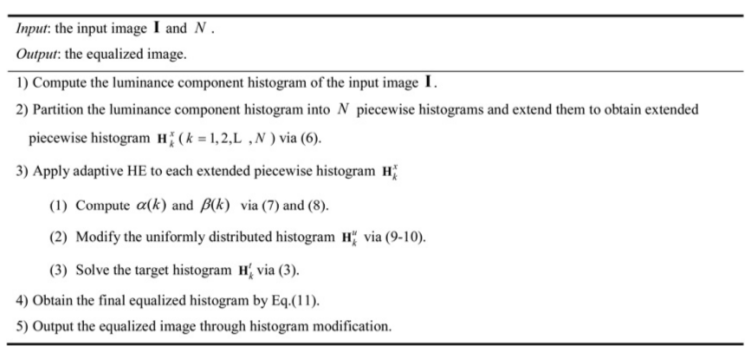
\includegraphics[width=\textwidth]{algoPaper.png}
    \caption{Algoritmo propuesto}
\end{figure}

El método llamado \textbf{AEPHE} toma como parámetro obligatorio de entrada la imagen y le aplica todas las transformaciones propuestas. Aparte, hay otros parámetros de entrada opcionales:
\begin{itemize}
\item \textit{Alphas:} Toma un vector de $\alpha$'s, los cuales serán aplicados en orden a cada subhistograma generado durante el algoritmo.
\item \textit{Betas:}  Toma un vector de $\beta$'s, los cuales serán aplicados en orden a cada subhistograma generado durante el algoritmo.
\item \textit{Gammas:} Toma un vector de $\gamma$'s, los cuales serán aplicados en orden a cada subhistograma generado durante el algoritmo.
\item \textit{number\textunderscore of\textunderscore histogramas:} Cantidad de histogramas en los que se desea partir el histograma original de la imagen de entrada. El valor es $3$ por defecto.
\item \textit{discretization\textunderscore bin\textunderscore width:} Cantidad de \textit{bins} en los que se dividirá el histograma al momento de realizar la conversión para trabajar con enteros o floats. El valor es $1/255$ (255 bins) por defecto. 
\item \textit{plot\textunderscore intermediate\textunderscore histograms:} Booleano que indica si se quiere ir mostrando las figuras de todos los subhitogramas generados durante la ejecución del algoritmo. El valor es \textit{False} por defecto.
\end{itemize}

La razón por la cual tomamos vectores de valores en algunos parámetros será explicada posteriormente cuando hablemos sobre la experimentación y los problemas con los que nos encontramos al realizar los mismos.

Si el vector de $\gamma$'s no se especifica, tomamos todos los valores como 0 ya que dicho parámetro no contribuye notablemente al realce de la imagen. Si alguno de los otro dos vectores (vector de $\alpha$'s o $\beta$'s) es nulo, luego se procede a calcularlos de la manera que lo indica el paper:

\begin{equation}
\alpha = \dfrac{M_{i}}{M_{i} + M_{c}}
\end{equation}
\begin{equation}
\beta = \dfrac{M_{c}}{M_{i} + M_{c}}
\end{equation}

\begin{figure}[H]
	\centering
    \begin{subfigure}{0.5\textwidth}
        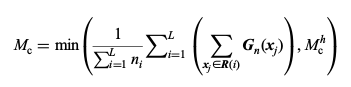
\includegraphics[width=0.9\textwidth]{calculo-Mc.png}
    \end{subfigure}\hfill
    \begin{subfigure}{0.5\textwidth}
        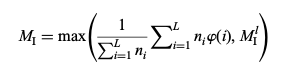
\includegraphics[width=0.9\textwidth]{calculo_Mi.png}
    \end{subfigure}\hfill
\end{figure}

Cada uno de estos valores se calcula para cada subhistograma generado.

\section{Experimentación}

Al realizar la experimentación, uno de los problemas con el que nos encontramos fue que en imágenes que poseían partes muy claras, estas secciones quedaban completamente negras al aplicarles nuestro algoritmo.  Por ejemplo, al utilizar una imagen tomada por nosotros, nos pasaba lo siguiente:

\begin{figure}[H]
	\centering
        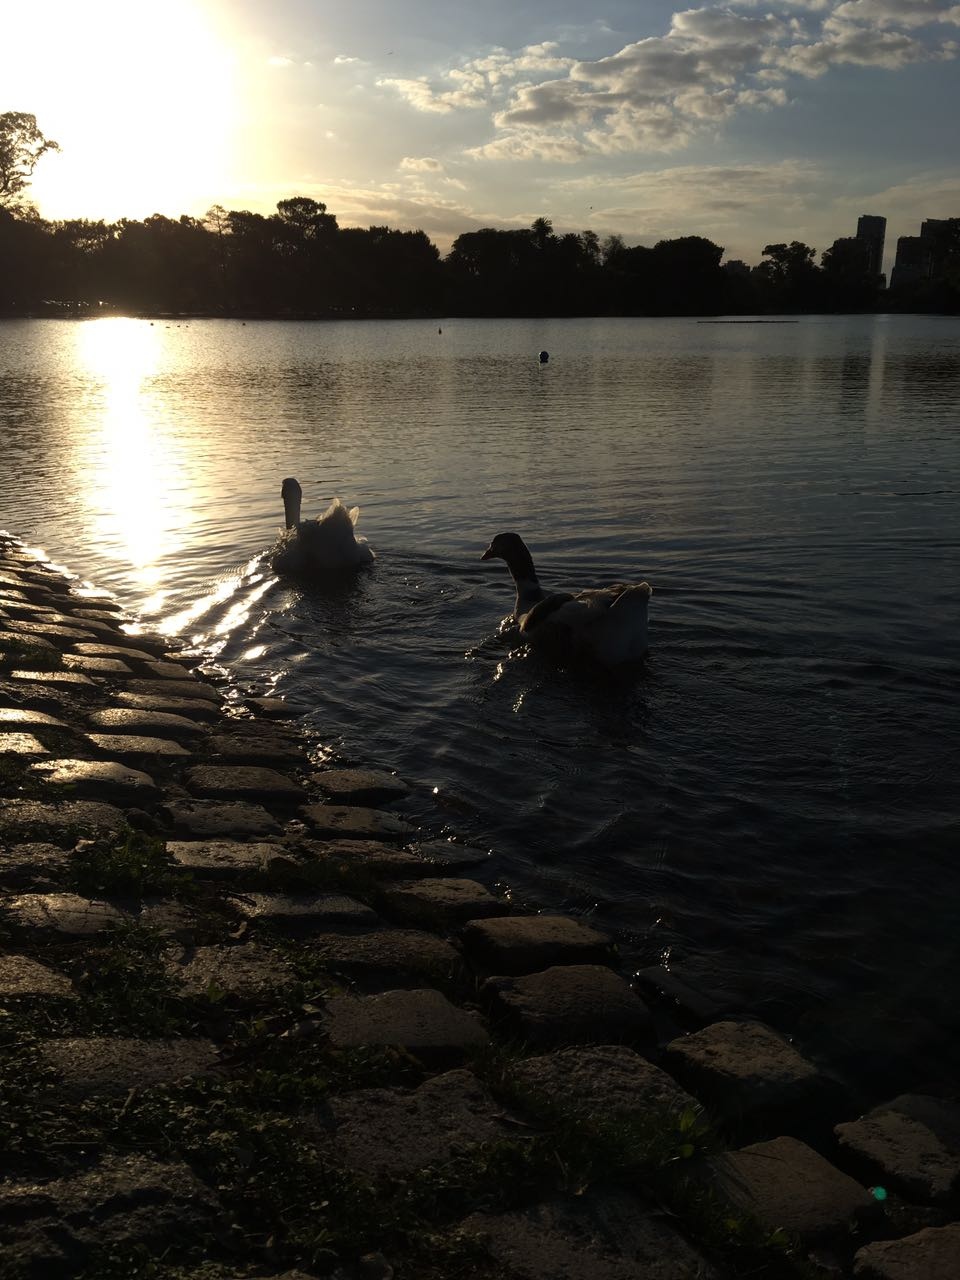
\includegraphics[width=0.4\textwidth]{patitos1.jpg}
        \caption{Imagen original}
\end{figure}
\begin{figure}[H]
	\centering
        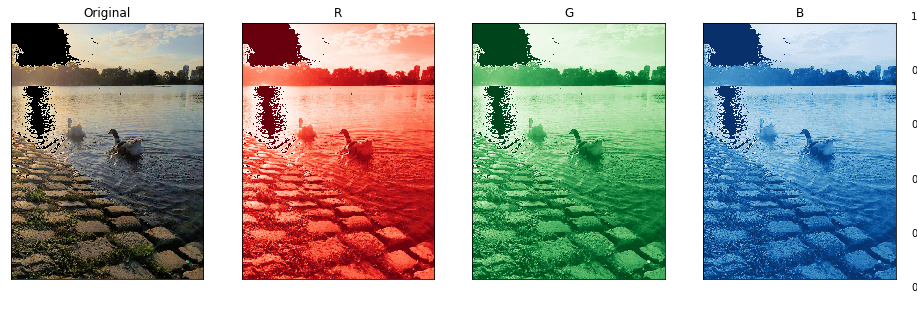
\includegraphics[width=0.9\textwidth]{patitos-alpha096-beta004-k3.png}
        \caption{Imagen ecualizada junto con sus canales R, G, B}
\end{figure}

Debido a esto, tomamos la decisión de que nuestro algoritmo tome como parámetros de entrada vectores de valores de $\alpha$ y $\beta$. Esto nos sirve para decidir qué peso darle al histograma uniforme y al original, lo cual se deduce de la fórmula provista:

\begin{figure}[H]
	\centering
        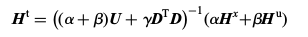
\includegraphics[width=0.5\textwidth]{calculo-H.png}
\end{figure}

\subsection{Variación de parámetro K}

Para esta parte buscamos experimentar variar el valor de K, el cual indica la cantidad de histogramas en los que se va a partir el original. 

\subsubsection{Experimento 1}

Para uno de los experimentos que decidimos realizar, tomamos una imagen que posee partes muy claras y el resto de la imagen un tanto oscuro en comparación y evaluamos cómo afecta la elección de dicho parámetro. Utilizamos el $\alpha$ y $\beta$ que se calcula automáticamente para cada subhistograma utilizando la fórmula del paper.

Obtuvimos los siguientes resultados:

\begin{figure}[H]
	\centering
        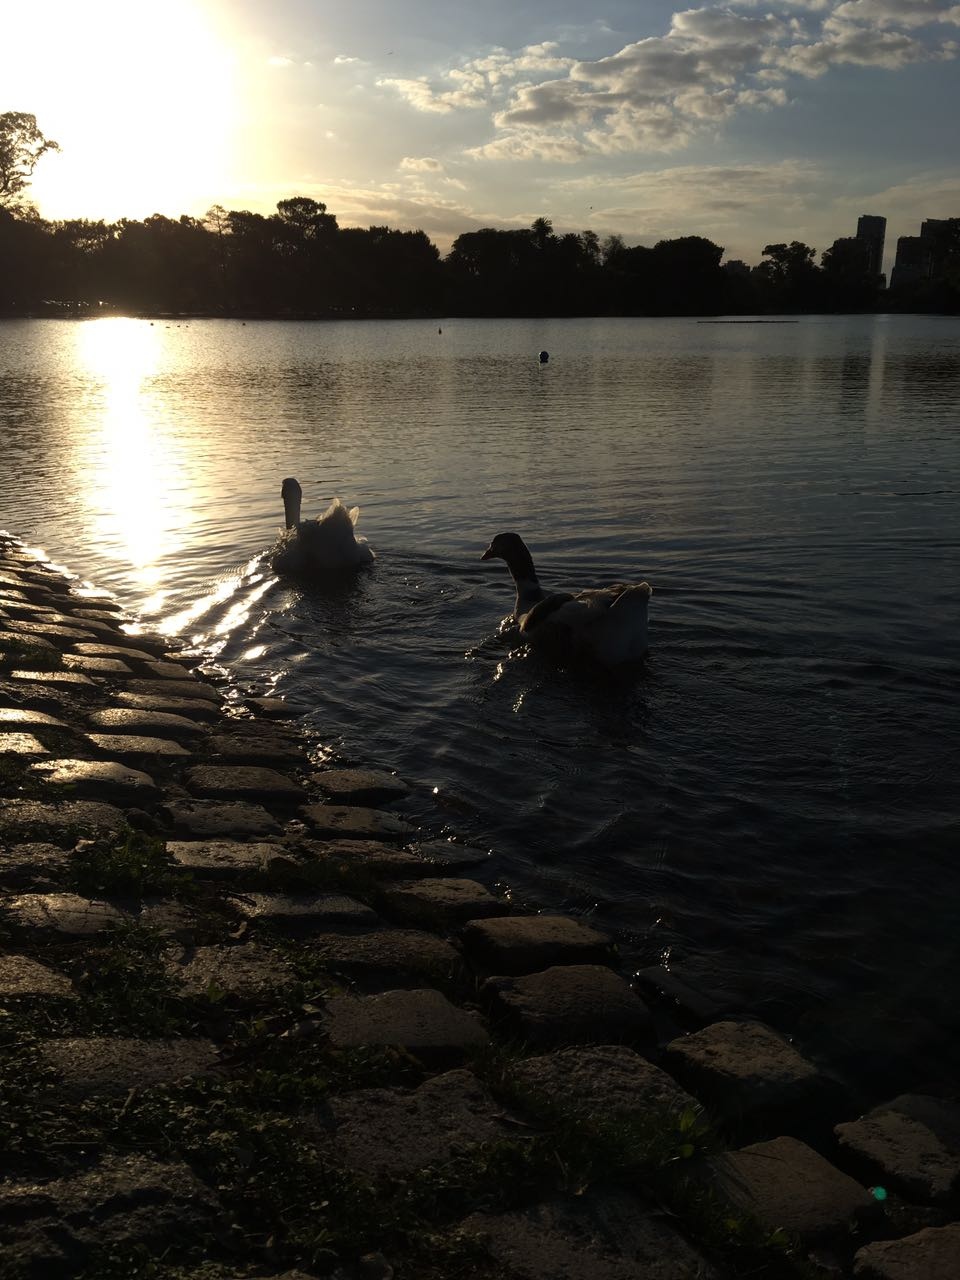
\includegraphics[width=0.3\textwidth]{patitos1.jpg}
        \caption{Imagen original}
\end{figure}

\begin{figure}[H]	
	\centering
    \begin{subfigure}{0.3\textwidth}
        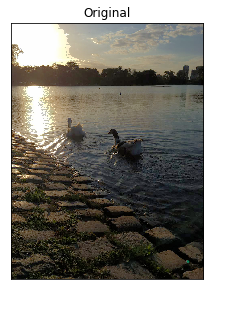
\includegraphics[width=0.9\textwidth]{patitos-k2.png}
        \subcaption{$k=2$}
    \end{subfigure}\hfill
    	\centering
    \begin{subfigure}{0.3\textwidth}
        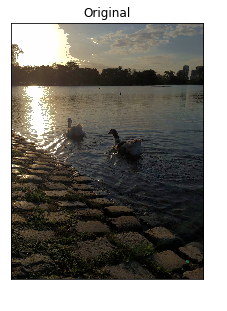
\includegraphics[width=0.9\textwidth]{patitos-k4.png}
        \subcaption{$k=4$}
    \end{subfigure}\hfill	
    \centering
    \begin{subfigure}{0.3\textwidth}
        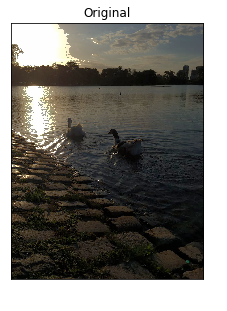
\includegraphics[width=0.9\textwidth]{patitos-k16.png}
        \subcaption{$k=16$}
    \end{subfigure}\hfill
\end{figure}

Al comparar las imágenes, se puede observar que a medida que se aumenta el $K$, la imagen se iba oscureciendo cada vez más. Debido a esto, nos fijamos en los histogramas de cada imagen:

\begin{figure}[H]
	\centering
        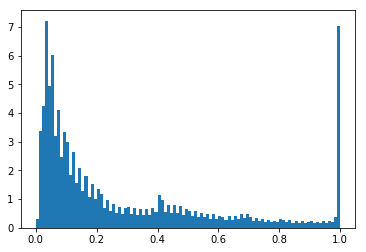
\includegraphics[width=0.3\textwidth]{patitos1-histogramaOriginal.png}
        \caption{Histograma de imagen original}
\end{figure}

\begin{figure}[H]	
	\centering
    \begin{subfigure}{0.3\textwidth}
        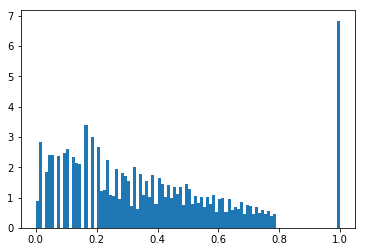
\includegraphics[width=0.9\textwidth]{patitos-histogramaFinal-k2.png}
        \subcaption{Histograma de imagen ecualizada con $k=2$}
    \end{subfigure}\hfill
    	\centering
    \begin{subfigure}{0.3\textwidth}
        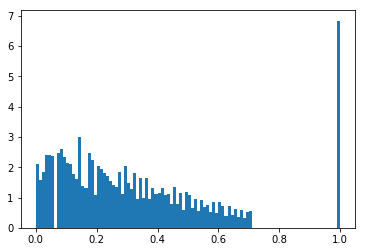
\includegraphics[width=0.9\textwidth]{patitos-histogramaFinal-k4.png}
        \subcaption{Histograma de imagen ecualizada con $k=4$}
    \end{subfigure}\hfill	
    \centering
    \begin{subfigure}{0.3\textwidth}
        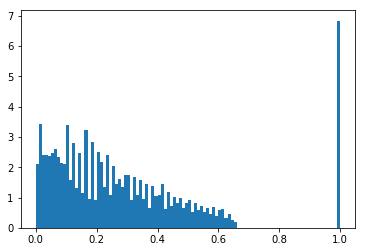
\includegraphics[width=0.9\textwidth]{patitos-histogramaFinal-k16.png}
        \subcaption{Histograma de imagen ecualizada con $k=16$}
    \end{subfigure}\hfill
\end{figure}

Así pudimos ver que en el caso de imágenes que poseen muchos píxeles oscuros y muchos claros, a medida que se va aumentando el valor de $k$, los histogramas tienden a ir concentrándose hacia el lado de estos valores elevados, en vez de generarse una ecualización equilibrada sobre todos los valores de gris. Esto mismo nos pasó con otras imágenes tomadas por nosotros que poseían características similares en cuanto a la distribución de colores. 

\subsubsection{Experimento 2}

Realizamos otros experimentos tomando imágenes provistas por la cátedra, cuya característica es que en su mayoría son oscuras y fijamos los parámetros $\alpha$ y $\beta$. Obtuvimos los siguientes resultados:

\begin{figure}[H]
	\centering
        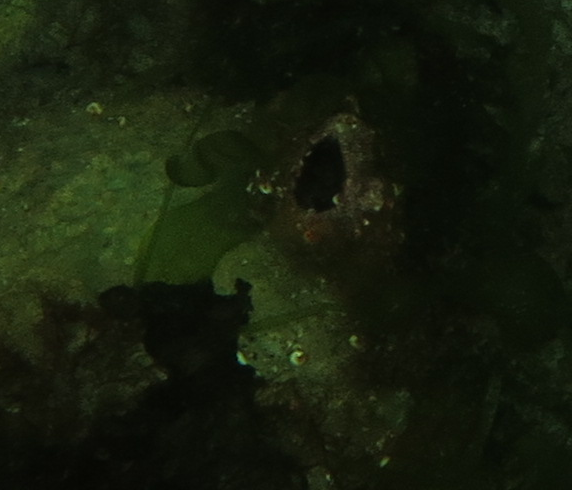
\includegraphics[width=0.3\textwidth]{1906ax.png}
        \caption{Imagen original}
\end{figure}

\begin{figure}[H]	
	\centering
    \begin{subfigure}{0.3\textwidth}
        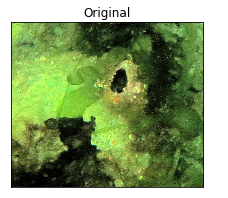
\includegraphics[width=0.9\textwidth]{1906ax-k2.png}
        \subcaption{$k=2$}
    \end{subfigure}\hfill
    	\centering
    \begin{subfigure}{0.3\textwidth}
        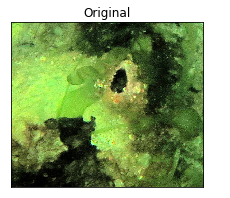
\includegraphics[width=0.9\textwidth]{1906ax-k4.png}
        \subcaption{$k=4$}
    \end{subfigure}\hfill	
    \centering
    \begin{subfigure}{0.3\textwidth}
        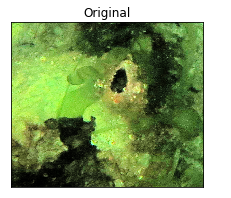
\includegraphics[width=0.9\textwidth]{1906ax-k16.png}
        \subcaption{$k=16$}
    \end{subfigure}\hfill
\end{figure}

Si bien se puede observar un leve cambio entre la imagen con $k=2$ y las demás, pudimos ver que a medida que se va aumentando el valor de $k$ para $k \geq 4$ no se producían cambios muy significativos.

\subsubsection{Experimento 3}

Realizamos un experimento similar al anterior (fijando el valor de $\alpha$ y $\beta$) con la imagen del primer experimento. Obtuvimos las siguientes imagenes:

\begin{figure}[H]
	\centering
        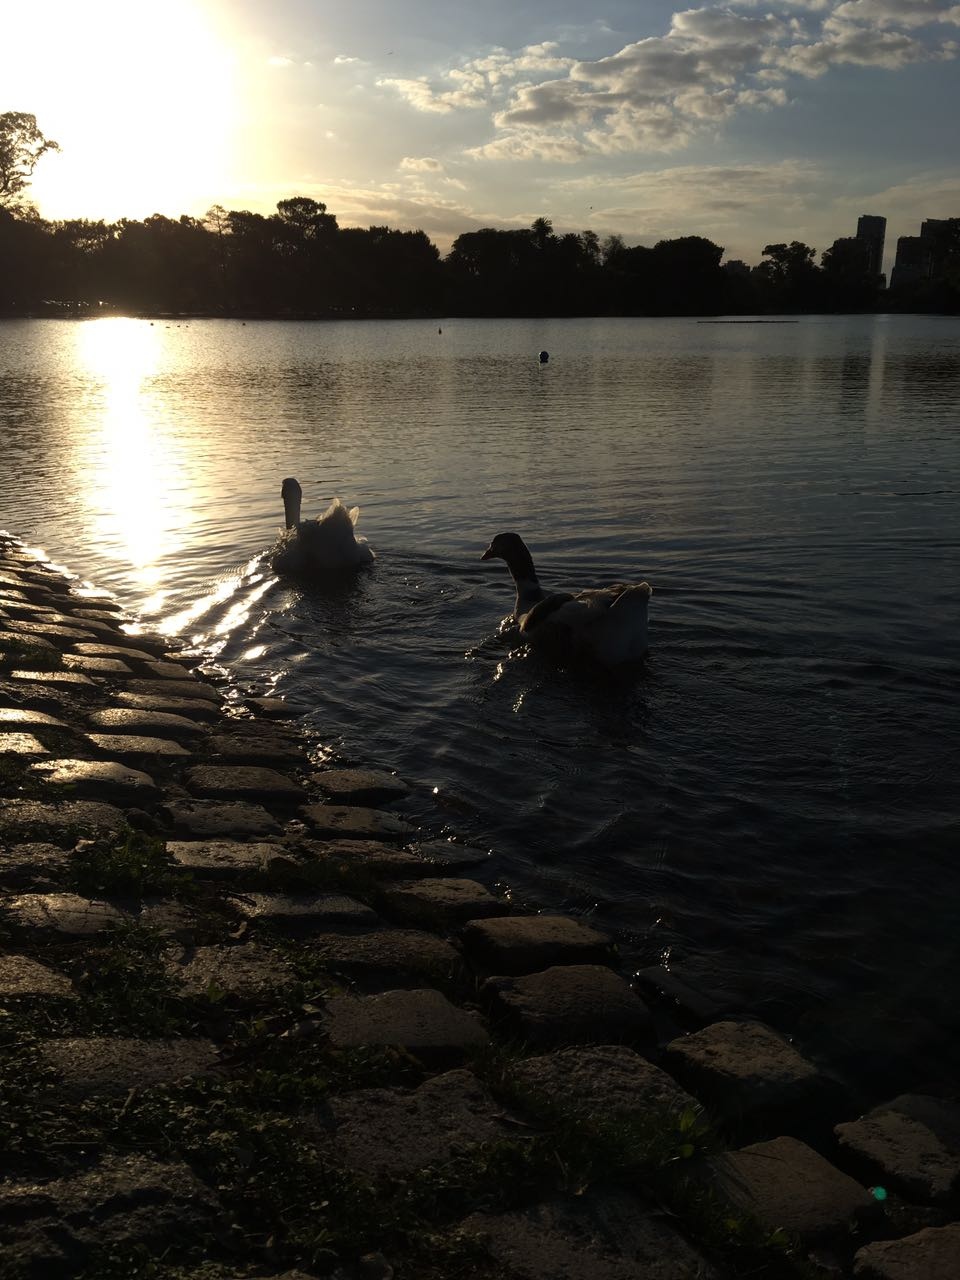
\includegraphics[width=0.3\textwidth]{patitos1.jpg}
        \caption{Imagen original}
\end{figure}

\begin{figure}[H]	
	\centering
    \begin{subfigure}{0.3\textwidth}
        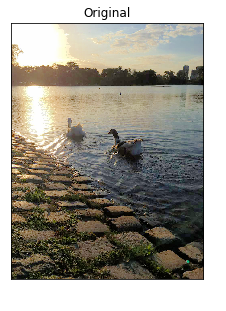
\includegraphics[width=0.9\textwidth]{patitos-alphabetafijos-k4.png}
        \subcaption{$k=4$}
    \end{subfigure}\hfill
    	\centering
    \begin{subfigure}{0.3\textwidth}
        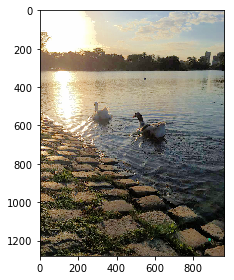
\includegraphics[width=0.9\textwidth]{patitos-alphabetafijos-k8.png}
        \subcaption{$k=8$}
    \end{subfigure}\hfill	
    \centering
    \begin{subfigure}{0.3\textwidth}
        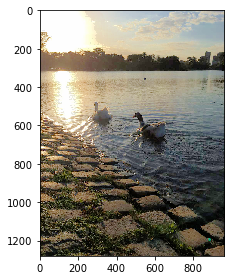
\includegraphics[width=0.9\textwidth]{patitos-alphabetafijos-k16.png}
        \subcaption{$k=16$}
    \end{subfigure}\hfill
\end{figure}

Acá podemos observar resultados similares que los del experimento anterior, por lo que concluímos que el $k$ no produce cambios significativos al dejar fijos el valor de $\alpha$ y $\beta$.

\newpage 

\begin{thebibliography}{9}
\bibitem{paper}
Zhigang Ling, Yan Liang, Yaonan Wang, He Shen, Xiao Lu. \textit{Adaptive extended piecewise histogram equalisation for dark image enhancement.} IET Image Processing. 2015.
\end{thebibliography}


\end{document}